\documentclass{article}

% if you need to pass options to natbib, use, e.g.:
% \PassOptionsToPackage{numbers, compress}{natbib}
% before loading nips_2016
%
% to avoid loading the natbib package, add option nonatbib:
% \usepackage[nonatbib]{nips_2016}

\usepackage[final]{nips_2016}

% to compile a camera-ready version, add the [final] option, e.g.:
% \usepackage[final]{nips_2016}

\usepackage[utf8]{inputenc} % allow utf-8 input
\usepackage[T1]{fontenc}    % use 8-bit T1 fonts
\usepackage{hyperref}       % hyperlinks
\usepackage{url}            % simple URL typesetting
\usepackage{booktabs}       % professional-quality tables
\usepackage{amsfonts}       % blackboard math symbols
\usepackage{nicefrac}       % compact symbols for 1/2, etc.
\usepackage{microtype}      % microtypography
\usepackage{graphicx}
\usepackage{subfigure}

\title{Project 1: Applying Convolutional Neural Networks on MNIST}

% The \author macro works with any number of authors. There are two
% commands used to separate the names and addresses of multiple
% authors: \And and \AND.
%
% Using \And between authors leaves it to LaTeX to determine where to
% break the lines. Using \AND forces a line break at that point. So,
% if LaTeX puts 3 of 4 authors names on the first line, and the last
% on the second line, try using \AND instead of \And before the third
% author name.

\author{
  Marcus ~Brenscheidt \\
  Heinrich Heine University\\
  \texttt{marcus.brenscheidt@uni-duesseldorf.de} \\
  %% examples of more authors
  \And
  Bastian Berndt \\
  Heinrich Heine University\\
  \texttt{bastian.berndt@uni-duesseldorf.de} \\
  \And
  Tobias Uelwer \\
  Heinrich Heine University\\
  \texttt{tobias.uelwer@uni-duesseldorf.de} \\
  %% \AND
  %% Coauthor \\
  %% Affiliation \\
  %% Address \\
  %% \texttt{email} \\
  %% \And
  %% Coauthor \\
  %% Affiliation \\
  %% Address \\
  %% \texttt{email} \\
  %% \And
  %% Coauthor \\
  %% Affiliation \\
  %% Address \\
  %% \texttt{email} \\
}

\begin{document}
%\nipsfinalcopy %is no longer used

\maketitle

\begin{abstract}
  In this short paper, we explore how to use convolutional neural networks for the MNIST challenge. Furthermore, we explore how the design of our network, as well as the choice of hyperparameters affects the performance of our CNN-approach. We will conclude with the proposal of a minimal CNN which represents an optimal tradeoff between complexity and prediction accuracy.
\end{abstract}

\section{Introduction to MNIST and Convolutional Neural Networks}
\subsection{Data}
In this paper we try to classify handwritten digits with convolutional neural network. Our dataset, which is known as MNIST, is commonly used in Machine Learning tutorials and competitions. MNIST is an acronym for Mixed National Institute of Standards and Technology database. This database is basically a collection of 28x28 greyscale pictures. For an example picture, please refer to figure \ref{acht}.

\begin{figure}[h]
\centering
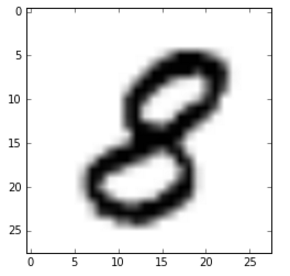
\includegraphics[width=0.35\textwidth]{imgs/8.png}
\caption{Handwritten eight from MNIST}\label{acht}
\end{figure}

\subsection{Why Convolutional Networks?}
Conventional Fully Connected Neural Network often fail to take local structure in our data into account. For a lot of machine learning tasks, we don't have spatial relationship between the dimsensions in our data points. However, this clearly does not hold true for Image Data, where the position of a pixel is almost as important as the value it holds.

Convolutional neural networks take spatial structure in our data into acount by learning and applying filters used for convolution in our neural networks. Oftentimes, we use convolutional filters as intermediary layers in our neural network architecture, and pass their output into conventional fully connected layers.

\section{Implementing a simple CNN for the MNIST challenge}
\subsection{Basic Architecture}
In this section, we will start with a prototypical CNN architecture, consisting of 2 convolutional layers, a fully connected layer and an output layer. The output of every layer (except from the output layer) is activated by a rectified linear unit. Furthermore, the output of each convolutional layer is max-pooled with windowsize 2 and stepsize 2. For a visualization of the architecture, please refer to figure \ref{std_graph}.

\subsubsection*{Convolutional Layers}
Our first convolutional layer consists of 32 5x5 kernels. Our second convolutional layer translates these 32 channels into 64 channels with 5x5 kernels. Each output is passed into a rectifier and then maxpooled. As a stepsize for convolution, we chose single steps.

\subsubsection*{Fully Connected Layer and Output Layer}
Finally, we apply a fully connected layer that connects the maxpooled output from our convolutional layers with our output layer. The fully connected layer has a size of 7*7*64x1024. The output layer translates these 1024 inputs to the 10 classes (numbers). It has a shape of 1024x10.

\begin{figure}
\centering
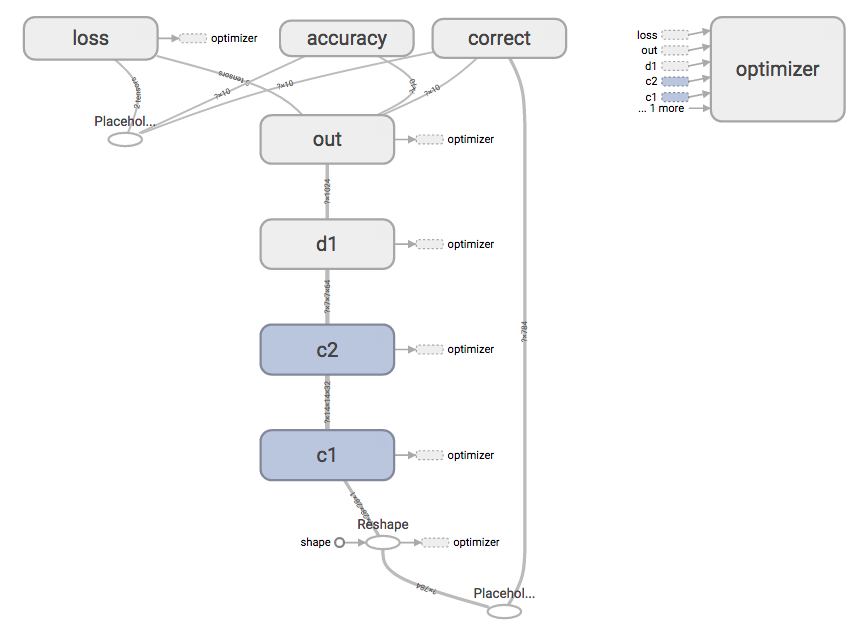
\includegraphics[width=0.7\textwidth]{imgs/std_graph.png}
\caption{Abstract representation of our computation graph, c: convolutional, d: fully connected}\label{std_graph}
\end{figure}

\subsection{Training Process}

For training our CNNs, we developed our own framework that allows rapid creation of different CNN architectures. Another central goal for our framework was logging and discoverability, so that we can easily compare and analyze the many different architectures that we want to test. Therefore we implemented tensorboard support, so that for any high level specification of a CNN, we can see the correct Graph in Tensorboard and have properly labeled, exhaustive statisticis, such as distributions, scalar summaries, and image summaries of misclassified inputs as well as convolved inputs.

For each CNN, we construct a proper prediction graph, with proper logging capabilities. This graph is then passed into a loss node, which, in turn, is passed into an optimization node. For optimization we used the Adam Optimizer.

The Adam Optimizer has empirically shown to be a rather good and stable optimizer. Further more, it allows us to ignore step size as a parameter.

\subsection{Evaluating Test Performance}
\subsubsection{Quantitative Performance Analysis}

In general, all of our tested Architectures achieved good results, hovering between 98 - 99 \% Accuracy on the test-set.

In rare cases, we even achieved accuracies higher than 99 \% with our standard configuration. Please refer to the plot below.

\begin{figure}[h]
\centering
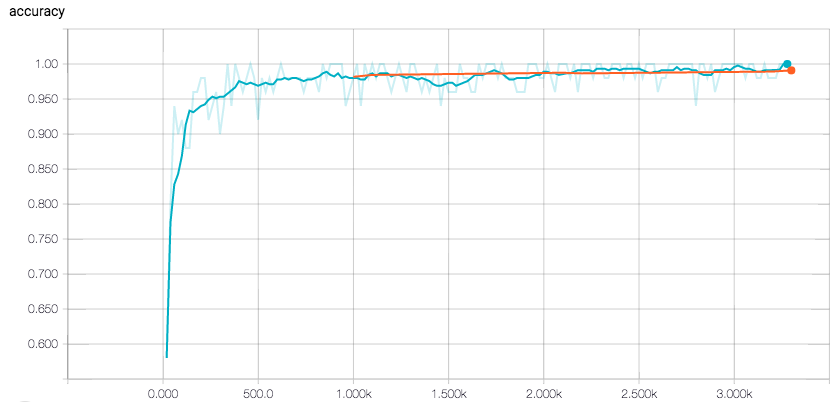
\includegraphics[width=0.7\textwidth]{imgs/accuracy_std.png}
\caption{Blue: Training Perfomance, Orange: Test Performance}
\end{figure}

For the performance measurement, we logged accuracy on our Training Set every 20th iteration step, while we measured the perfomance on the whole test set only every 1000th iteration. Overall, we performed our tests over the range of 3 epochs. 

However, we usually see the trend in our performance evaluations, that most neural network architectures with sufficient complexity perform equivalently good, with 98.XX \% accuracy after a few epochs.

\subsubsection{Qualitative Performance Analysis}

Aside from a quantitative analysis, which only looks at the raw accuracy achieved by a neural network, we also try get a \textit{qualitative} understanding of how our networks performs. This can be done by investigating which subsets of the testdata gets misclassified. A subset of the misqualified inputs is represented in figure \ref{misclassified}.

On closer inspection, we can see that our misclassified samples are rather irregular representations of their respective numbers and might even be ambiguous for the human perception (5 vs. 3, last image).

\begin{figure}
\centering
\begin{tabular}{cc}
  
\includegraphics[width=0.27\textwidth]{imgs/mis1.png}    
\includegraphics[width=0.27\textwidth]{imgs/mis2.png}    
\includegraphics[width=0.27\textwidth]{imgs/mis3.png} \\
 
\includegraphics[width=0.27\textwidth]{imgs/mis4.png}    
\includegraphics[width=0.27\textwidth]{imgs/mis5.png}    
\includegraphics[width=0.27\textwidth]{imgs/mis6.png} \\

\includegraphics[width=0.27\textwidth]{imgs/mis7.png}    
\includegraphics[width=0.27\textwidth]{imgs/mis8.png}    
\includegraphics[width=0.27\textwidth]{imgs/mis9.png} \\
\end{tabular}
\caption{9 Misclassified Images from our Testset}\label{misclassified}
\end{figure}

\section{Effect of Architecture and Hyperparameters on performance}


\subsection{Preface: On Randomness and Determination in Neural Network training}
Training Neural Networks is usually not a deterministic process. While the optimization algorithms themselves are often deterministic, Initialization of the layer Variables usually follows some random distributions.


\subsection{Effect of Iteration Count}
Optimization of Neural Networks is usually done by some form of gradient descent. Gradient Descent follows a decline in a loss function and thus seeks some form of localized minimum. This means that during the optimization process, our network configuration converges against a local minimum.

Thus, increasing Iteration Count has a beneficial effect on accuracy, as long as we haven't yet converged against our optimal configuration. However, one can observe diminishing returns once the optimization process has reached a loss minimum. Increasing Iteration Count does not allow us to improve the accuracy of our predictions beyond a certain threshold, which is determined by our network architecture and a little bit of chance (since the local maximum we find is dependent on our starting point).

\subsection{Effect of Batch-Size during Training Process}
We ran an empirical investigation into the optimal setting of the Batch-Size. We tested batchsizes between 10 and 5000 and averaged each over 5 trials. Each trial consisted of training 1 initial epoch where we measured final accuracy and computation times.

\begin{figure}[h]
\centering
\subfigure{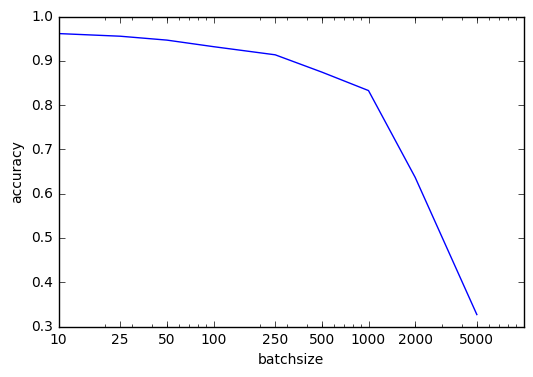
\includegraphics[width=0.45\textwidth]{imgs/acc_vs_batchsize.png}}
\subfigure{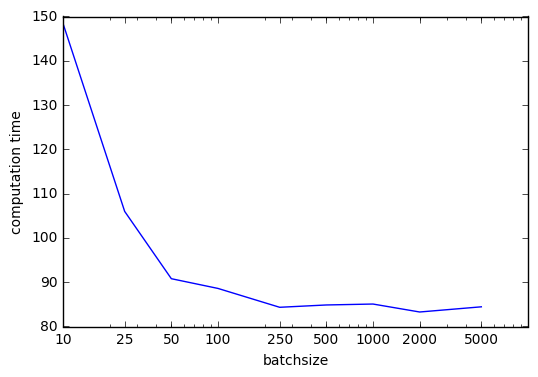
\includegraphics[width=0.45\textwidth]{imgs/time_vs_batchsize.png}}
\caption{Batchsize plotted against Accuracy and Computation time for one epoch.}\label{batchsizes}
\end{figure}

For a plot of our results, please refer to \ref{batchsizes}.
We can see that the accuracy degrades slowly with a growing batchsize, while the computation time reduces rather fast with bigger batches.

From these experiments we concluded an optimal batch-size of 50 for our training process.


\subsection{Effect of Learning Rate on the Optimization Process}

Since we used the Adam Optimizer, the learning rate didn't have quite the same impact on our performance compared to more conversative stochastic gradient descent algorithms.

The Adam Optimizer adjusts the step size dynamically based on adaptive estimations of lower order moments of our cost-function. Thus setting an initial step-size does only have a minor influence on the actual steps being made in the optimization process. More information can be  found in [2].

\subsection{Effect of Pooling}
Pooling is both a tool for reducing the dimensionality of our feature set, but can also be seen as rectifier unit in the sense that it introduces nonlinearity into the functions computable by a neural network [1].

In our tests, early pooling has shown to reduce computation times by quite a margin. For pooling, we relied exclusively on Max-Pooling, which was applied to part of our Convolutional Layers. Stride and filter-size, were both set to 2, which translates to only picking the maximum signal from mutually exclusive 2x2 patches.

If we leave out the pooling layers completely, we can observe, that the time required for the optimization process  increases noticably. Furthermore, we have the additional downside that our network tends to overfit.

\subsection{Effect of general network shape on Learning}
Even with a small number of hidden layers and convolutional layer, we get rather close to a practical threshold of 99\%. We presume that the issue with achieving a higher accuracy lies not within a lack of theoretical complexity representable through our Neural Networks, but rather in the irregularities in the data itself and a small number of outliers.

When adding more convolutional layers or fully connected layers, we hardly see a noticable improvement in accuracy. However, deeper networks and more variables require more computations for the optimization process. Adding more and/or wider layers mainly increases computation time per epoch while decreasing rate of convergence, however leading to a similar absolute outcome in terms of accuracy.


\section{Designing a minimal efficient CNN}

We measured the size of a network through the number of Variables that are optimized as a Key Performance Indicator.

Other possible metrics could also consider layer depth and diversity of layer types, as well as the usage of activation functions and pooling layers.

 To minimize the number of parameters, we relied primarily on small convolutional filters, which were then maxpooled in order to reduce the size of our final fully connected layer.

Our chosen minimal architecture consists of 5 layers in total. We start with 3 convolutional layers, each followed by a maxpool layer. The result is then passed into 1 fully connected layer, which is, again, passed into the final output layer.

\begin{center}
\begin{tabular}{l c c c c}
 \textbf{type} & \textbf{weights} & \textbf{bias} & \textbf{activation} & \textbf{\# parameter} \\
\midrule
convolutional & 3x3x1x4 & 4  & Rectifier, Maxpool2d & 40 \\
convolutional & 3x3x4x8 & 8 & Rectifier, Maxpool2d & 296 \\
convolutional & 3x3x8x4 & 4 & Rectifier, Maxpool2d & 292 \\
fully connected & 64x8 & 8 & Rectifier & 520 \\
out & 8x10 & 10 & Rectifier & 90 \\
\midrule
\textbf{total} & & & & \textbf{1238}
\end{tabular}
\end{center}

From the table, we can see that our minimal design only uses $1238$ Variables. With this size, we can achieve an accuracy greater than $95\%$. 

\begin{figure}[h]
\centering
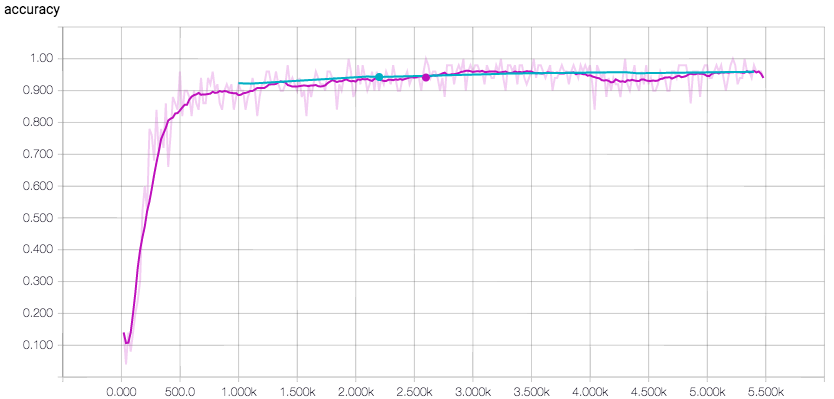
\includegraphics[width=0.7\textwidth]{imgs/acc_min.png}
\caption{Minimal Network, Blue: Training Perfomance, Orange: Test Performance}
\end{figure}

After 5 epochs of training, we finally reached an accuracy of $96.01\%$ on our testset.

This experiment has shown, that Convolutional Neural Networks are able to achieve quite good performance, even with a very limited amount of hidden variables and thus, limited complexity in the structure of our predictions.f


\section*{References}

References follow the acknowledgments. Use unnumbered first-level
heading for the references. Any choice of citation style is acceptable
as long as you are consistent. It is permissible to reduce the font
size to \verb+small+ (9 point) when listing the references. {\bf
  Remember that you can use a ninth page as long as it contains
  \emph{only} cited references.}
\medskip

\small

[1] Montufar, G. F., Pascanu, R., Cho, K., \& Bengio, Y. (2014). On the number of linear regions of deep neural networks. In Advances in neural information processing systems (pp. 2924-2932).

[2] Kingma, D., \& Ba, J. (2014). Adam: A method for stochastic optimization. arXiv preprint arXiv:1412.6980.

\end{document}
